% !TEX root = ../thesis.tex

\chapter{Pravdepodobnostný model kvantového výpočtu - návrh a realizácia}

Cieľom je vytvoriť v jazyku Haskell model, ktorý by dokázal merať stavy
kvantových bitov aj bez ich kolabovania. Na rozdiel od IBM Quantum
Experience tento model môže realizovať unitárne operácie aj paralelne.

\begin{figure}
	\centering 
	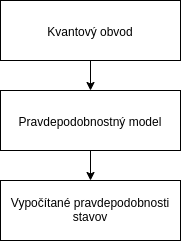
\includegraphics[width=.2\textwidth]{figures/navrh.png} 
	\caption{Konceptuálny návrh programu}
    \label{navrh}
\end{figure}


Pri pohľade na jednoduchý konceptuálny model (obrázok \ref{navrh}) je zrejmé
čo cheme dosiahnuť. Na vstupe je očakávaný kvantový obvod. Samotný program
prebehne tímnto obvodom ako interpreter a zároveň pomerá stavy na daných
miestach v obvode. Nakoniec vypíše výstup v zrozumiteľnej podobe.

\section{Definícia vstupu}

Celý kvantový obvod je možné rozdeliť do vertikálnych blokov alebo levelov.
Každý level obsahuje hradlá, ktorých počet je maximálne rovný počtu 
kvantových bitov, s ktorými daný obvod pracuje. Ak v danom levely nechceme
aplikovať žiadnu operáciu nad bitom, môžme definovať prázdny element.

Čiže kvantový obvod môžeme definovať ako list levelov, pričom level je datová
štruktúra, ktorá obsahuje list hradiel. Okrem hradiel každý level bude
obsahovať prepínač, ktorý siganlizuje či má nastať meranie po aktivácií 
hradiel v leveli.

\section{Pravdepodobnostný model}

\begin{figure}
	\centering 
	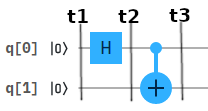
\includegraphics[width=.4\textwidth]{figures/circuit3.png} 
	\caption{Kvantový obvod s previazanými kvantovými bitmi.}
    \label{obvod}
\end{figure}

Pravdepodobnostný model možno vo funkčnosti prirovnať k interpreteru
kvatového obvodu. Tak ako bolo spomenuté v Pravdepodobnostnej analýze 
(kapitola \ref{pravAnalL}) je nutné brať v úvahu previazané a nepreviazané
kvantové bity. Previazanie je možné dosiahnuť hradlom CNOT (respektíve
C\textsuperscript{n}NOT). Našim cieľom nie je vytovoriť dokonalý interpreter,
z tohto dôvodu budeme využívať zjednodušené verzie týchto hradiel. Čo znamená,
že ak kontrólne bity sú v stave \(\ket{1}\) tak cieľový kvantový bit bude 
preklopený hradom \(X\). V inom prípade nenastane zmena v stavoch.


Pravdepodbnostný model si uchováva stavy všetkých kvantových bitova 
v stromovej štruktúre. Pri prechode levelom si uloží nové stavy do listov
tohto stromu. Ak sa v leveli nachádzajú len običajné hradlá, vzniká len
jediný nový list. Rozdiel nastáva pri prechode hradlom CNOT. Je zrejmé, že 
toto hradlo musí rozvetvovať stromovú štruktúru na dva podstromi. Každý z 
podstromov je označený pradvdepodobnosťou, s akou môže nastať daná zmena 
stavov. 

Pri meraní (fiktívnom meraní) sa spočítajú pravdepodobnosti všetkých listov
stromu a výsledky sa uložia do listu. Pre lepšie pochopenie funkčnosti 
programu opíšeme príklad. Majme kvantový obvod, ktorý je definovaný na 
obrázku \ref{obvod}. Na vstupe máme dva kvantové bity v stavoch \(\ket{0}\).
Definujme všetky potrebné datové štruktúry v jazyku Haskell. 

\begin{code}
l1 = Level [E, E] True
l2 = Level [H, E] True
l3 = Level [Cc, Ct] True
c = [l1, l2, l3]
st = StateTree 1 [q0, q0] []
rt = RT st []
\end{code}

Chceme merať v troch časových okamihoch, čo dosiahneme definovaním levelov
l1, l2 a l3. Každý level je označený na meranie pomocou True a využité hradlá
sú nasledovné:
\begin{itemize}
    \item E - prázdne
    \item H - Hadamardovo hradlo
    \item Cc - Kontrólny bit (angl. control bit) hradla CNOT
    \item Ct - Cieľový bit (angl. target bit) hradla CNOT
\end{itemize}

Pre ďalšie spracovanie spojíme levely  do jedného obvodu \(c\). Na ukladanie
stavov slúži stromová štruktúra StateTree. Jej definovaním hovoríme, že
počiatočné stavy sú q0, čo je označenie pre stav \(\ket{0}\). Pravdepodobnosť
dosiahnutia týchto stavov je 1 a zatiaľ neexistujú žiadne podstromi. Štruktúra
RT slúži na ukadanie výsledkov meraní. Spustením pravdepodobnostného modelu
dostaneme výslednú tabuľku typu RT.

\begin{code}
processRT = processCircuit c rt
\end{code}

\begin{figure}
	\centering 
	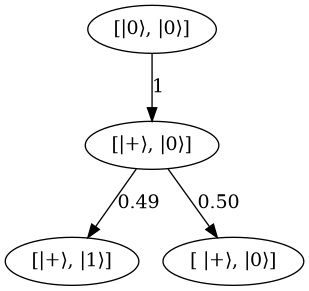
\includegraphics[width=.4\textwidth]{figures/ST.png} 
	\caption{Strom stavov (StateTree) po vykonaní kvantového obvodu.}
    \label{stateTree}
\end{figure}

To ako sa menili stavy kvantových bitov môžeme vidieť na obrázku
\ref{stateTree}. Je zrejmé, že využitím operácie Hadarmardovho hradla nenastane
vetvenie stromu stavov. To isé ale už neplatí pre hradlo CNOT. Nakoľko stav
kontrólneho bitu \(\ket{+}\) má \(50\%\)-tnú šancu skolabovať do stavu 
\(\ket{0}\) ako aj do stavu \(\ket{1}\), tak je prirodzené, že strom stavov 
sa rozvetví a každý podstrom má pravdepodobonsť dosihuntia približne \(0.5\).

Pri výpočte výsledkov je nutné započítať nie len pravdepodobnosti kolabovania
výsledných stavov ale aj pravdepodobnosti dosiahnutia podstromov, v ktorých 
sa dané stavy kvantových bitov nachádzajú. Meriame pravdepodobnosti kolabovania
bitov do stavov \(\ket{0}\) a \(\ket{1}\). Ide o dva stavy takže počet
kombinácií výsledkov je \(2^n\), kde \(n\) je počet kvantových bitov v obvode.
Teda pre dva bity možné kombinácie sú \(\ket{00}, \ket{01}, \ket{10}\) a
\(\ket{11}\). Vypočítajme výsledky pre level l3, čiže vychádzame z listov 
finálneho stromu stavov. Pre prvý list pravdepodobnosť dosiahnutia stavu:

\begin{itemize}
    \item \(\ket{00}\) je \(|\alpha_0\alpha_1|^2 = |\binom{1}{\sqrt{2}} \times
0|^2 = 0\)
    \item \(\ket{01}\) je \(|\alpha_0\beta_1|^2 = |\binom{1}{\sqrt{2}} \times
1|^2 = 0.5\)
    \item \(\ket{10}\) je \(|\beta_0\alpha_1|^2 = |\binom{1}{\sqrt{2}} \times
0|^2 = 0\)
    \item \(\ket{11}\) je \(|\beta_0\beta_0|^2 = |\binom{1}{\sqrt{2}} \times
1|^2 = 0.5\)
\end{itemize}

Pre druhý list obdobne platí to isté. Samozrejme treba započítať aj
pravdepodobnosť vykonania podstromu. Čiže všetky tieto pravdepodobnosti
kolabovania je nutné vynásobiť príslušnými hodnotami. Teda dostávame výsledky:
\begin{itemize}
    \item \(\ket{00}\) dosiahneme s pravdepodobnosťou \(0.25\)
    \item \(\ket{01}\) dosiahneme s pravdepodobnosťou \(0.25\)
    \item \(\ket{10}\) dosiahneme s pravdepodobnosťou \(0.25\)
    \item \(\ket{11}\) dosiahneme s pravdepodobnosťou \(0.25\)
\end{itemize}
